\section{Manage your hardware configuration}
\subsection{How virtual manager works}

\begin{frame}{Example of R and package installation}{hardware virtualisation}
\begin{columns}
\column{.5\textwidth}
\begin{itemize}[<+->]
	\item If we want a software from a different OS ?
	\item Use virtual machines
	\item Each application get a total different and independant environment
	\item Virtual machine could be transfered to another computer
\end{itemize}
\column{.5\textwidth}
\begin{itemize}[<+->]
	\item Redundancy between VMs
	\item Heavy to set up
	\item No automation
\end{itemize}
\end{columns}
\onslide<1-3>{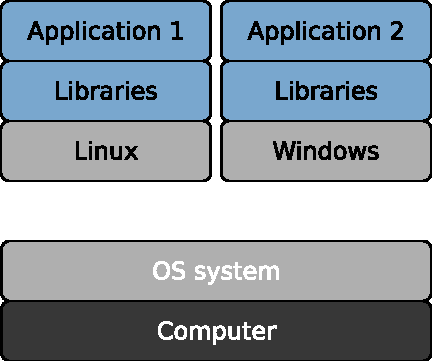
\includegraphics[width=0.3\textwidth]{images/VM_env_1.pdf}}
\onslide<2-3>{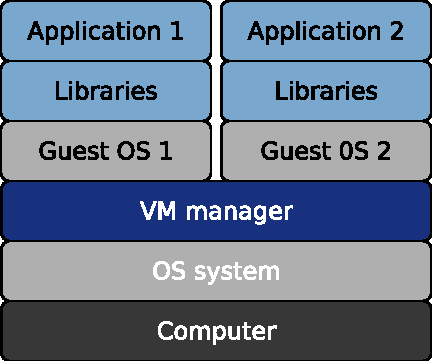
\includegraphics[width=0.3\textwidth]{images/VM_env_2.pdf}}
\end{frame}
\begin{frame}
\centering{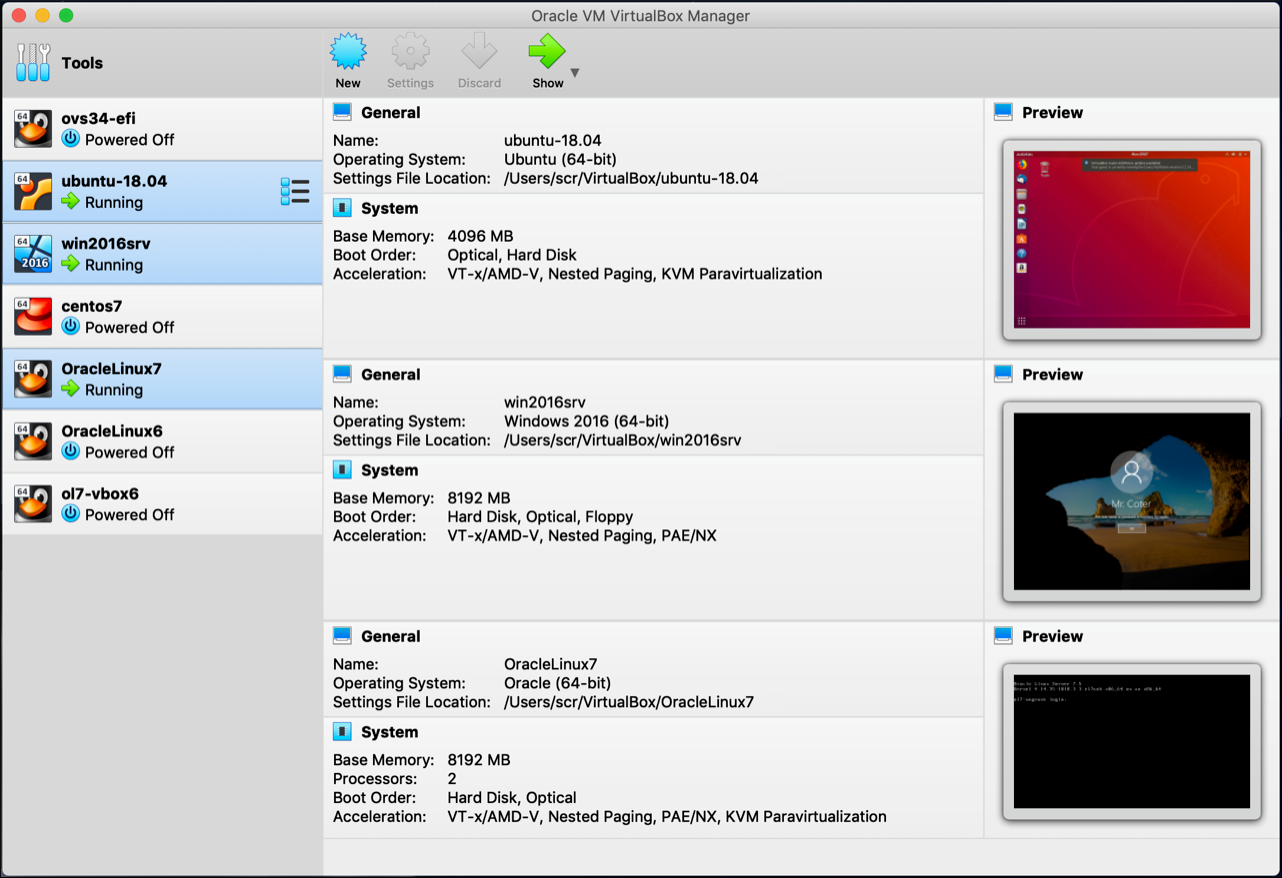
\includegraphics[width=0.8\textwidth]{images/virtualbox-main.png}}
\end{frame}

